\documentclass{article}
\usepackage[utf8]{inputenc}
\usepackage{tikz}

\title{HW 8 - Tikz}
\author{Amanda Mengotto}
\date{December 2015}

\usepackage{natbib}
\usepackage{graphicx}

\begin{document}

\maketitle

\section{Homework 8 Tikz}
This is the last part of question 4.

\begin{figure}
  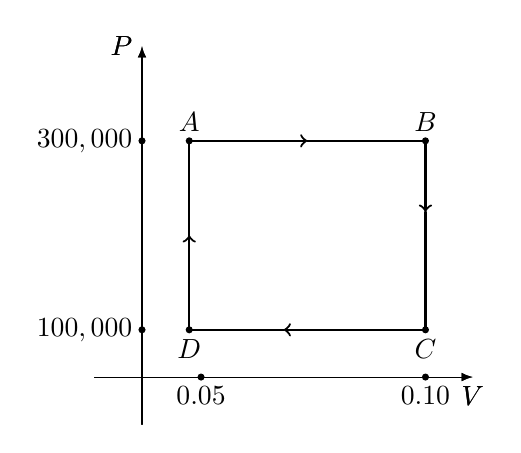
\begin{tikzpicture}
    [line cap=round,line join=round,x=2cm,y=2cm, scale=1.5, decoration={brace,amplitude=2pt}]

  \fill[black] (0.2,1) circle (0.3mm) node [anchor=south ,scale=1] {$ A$};
   \fill[black] (1.2,1) circle (0.3mm) node [anchor=south,scale=1] {$ B$};
 
 \fill[black] (0,1) circle (0.3mm) node [anchor=east ,scale=1] {$300,000$};
   
    \fill[black] (0.25,0) circle (0.3mm) node [anchor=north ,scale=1] {$ 0.05$};
     \fill[black] (1.2,0) circle (0.3mm) node [anchor=north ,scale=1] {$0.10$};
      
  \draw[-latex,color=black,thin] (-0.2,0) -- (1.4,0) node [anchor=north ,scale=1] {$V$};
   \draw[-latex,color=black,thin] (0,-0.2) -- (0,1.4)node [anchor=east ,scale=1] {$P$};

\draw[->,color=black,thick] (0.2,1) -- (0.7,1);
\draw[color=black,thick] (0.7,1) -- (1.2,1);        
\draw[->,color=black,thick](0.2,0.6) --  (0.2,1)(0.2,0.6);
\draw[color=black,thick] (0.2,0.6) -- (0.2,0.2);
\draw[->,color=black,thick] (1.2,1) -- (1.2,0.7);
\draw[color=black,thick] (1.2,0.7) -- (1.2,0.2);
\draw[->,color=black,thick] (1.2,0.2) -- (0.6,0.2);
\draw[color=black,thick] (0.6,0.2) -- (0.2,0.2);
 
  \fill[black] (1.2,0.2) circle (0.3mm) node [anchor=north ,scale=1] {$ C$};
   \fill[black] (0.2,0.2) circle (0.3mm) node [anchor=north,scale=1] {$ D$};

 \fill[black] (0,0.2) circle (0.3mm) node [anchor=east ,scale=1] {$100,000 $};

  \draw[-latex,color=black,thin] (-0.2,0) -- (1.4,0) node [anchor=north ,scale=1] {$V$};
   \draw[-latex,color=black,thin] (0,-0.2) -- (0,1.4)node [anchor=east ,scale=1] {$P$};

 \end{tikzpicture}
\end{figure}

\end{document}
